\section{Fault Injection using Hardware Tools}
Returning to hardware-based fault injection techniques, these days researchers may use several methods for introducing faults to a system. One such methodology uses EMP (Electromagnetic Pulse) devices to generate pulses strong enough to interfere with the logic of modern electronics. An example of such a device can be seen in Figure \ref{fig:emp_device}. \\

\begin{figure}[htbp]
    \centering
    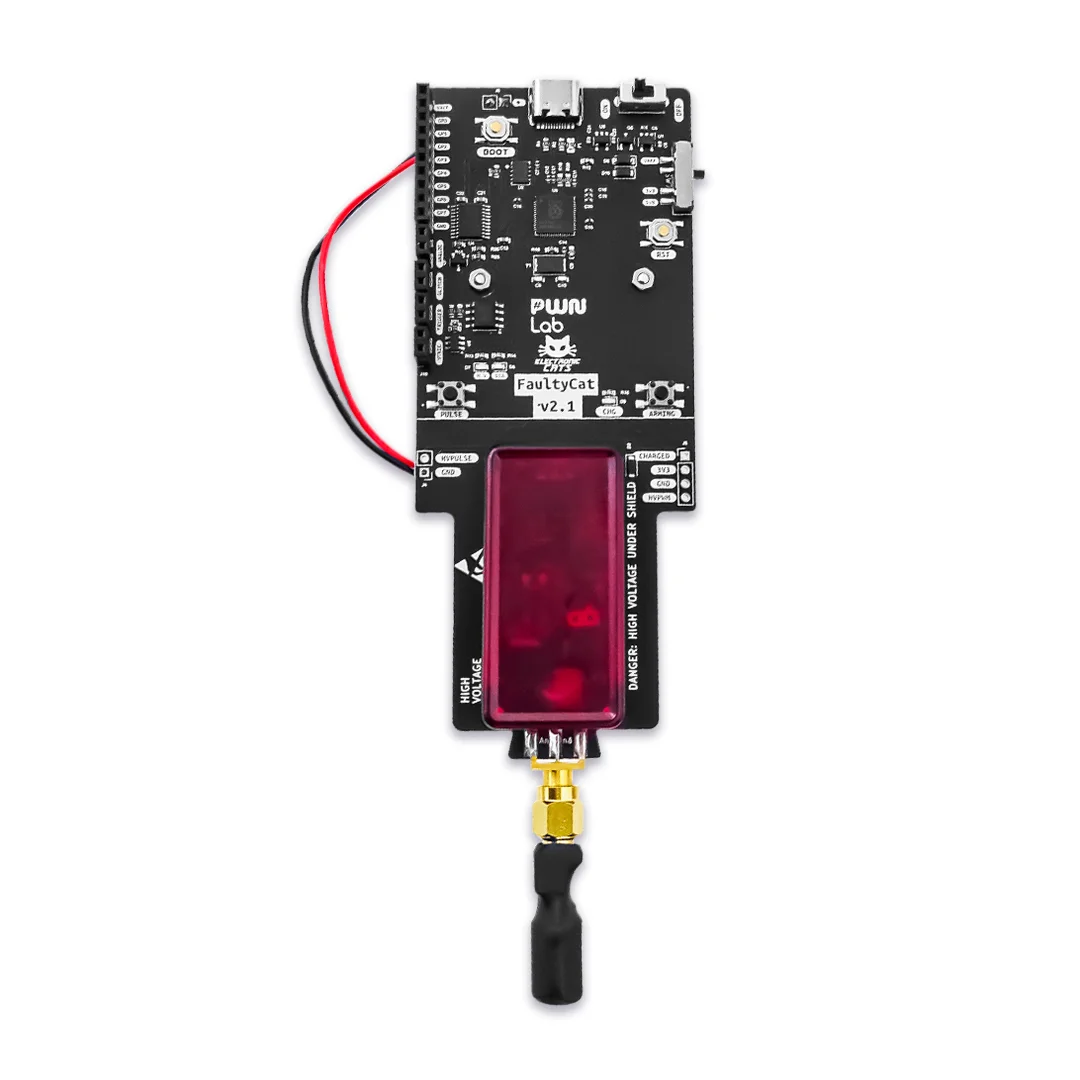
\includegraphics[width=0.5\linewidth]{assets/faultycat.png}
    \caption{EM Fault Injection Device}
    \label{fig:emp_device}
\end{figure}

Another hardware-based fault injection method utilizes the broad capabilities of an FPGA system, especially programmed to disrupt the signals of the components that manufacturers want to test, by being connected to them. These sub-systems are capable of modifying memory addresses in a program as well as cause pseudo-randomized bit-flips. Using FPGAs, researchers are capable of producing both SEUs and MBUs, as well as cause clock glitches, or even power glitches, all of which are broadly observed in areas such as space exploration or aviation. \\

These techniques can be applied in both conventional Von-Neumann processors like the ones commonly found in smartphones, as well as other FPGAs systems. In the case of fault injection in FPGA systems, it is also possible to reserve a portion of the system's maximum utilization for injecting faults, as previously discussed.

\subsection{Hardware Fault Injection using FISH}
Focusing in more detail on hardware-based fault injection using FPGAs, \textit{FISH} (Fault Injection Self-test Hardware) is a method proposed by Shandilya, Rahul, and Sharma, R.\cite{HardwareSite} and aims to create self-testing hardware, able to effectively inject MBU faults into the rest of the system. The proposed implementation consists of 4 8-bit LFSRs (Linear Feedback Shift Registers) that are tasked with creating a pseudo-randomized string of numbers that will determine which bits in the memory are flipped during the fault injection process. A programmable LFSR circuit can be viewed in Figure \ref{fig:lfsr}. \\

\begin{figure}[htpb]
    \centering
    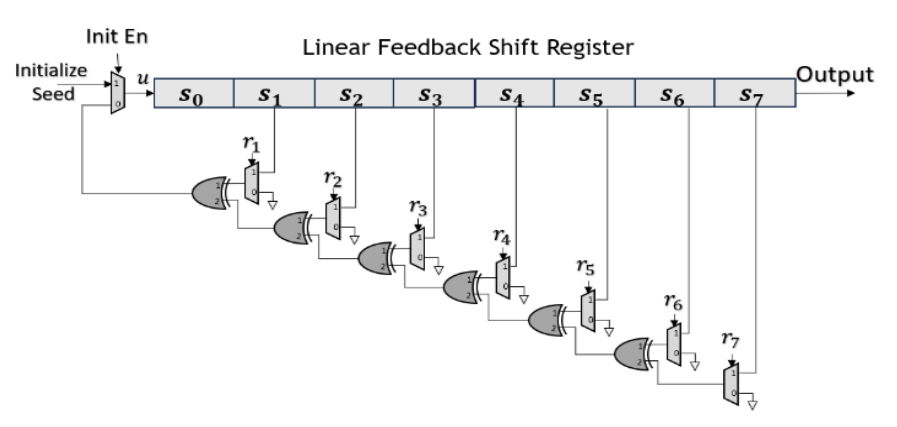
\includegraphics[width=0.9\linewidth]{assets/lfsr_circuit.png}
    \caption{Programmable LFSR Circuit}
    \label{fig:lfsr}
\end{figure}

As stated in the paper, the LFSRs functions by initially using a seed as a base number sequence, and shifting its values while using the previous outputs of the register as new inputs to determine how much a number is going to be shifted, generating whitening sequences,
pseudo-noise sequences, pseudo-random numbers, etc. \\

The complete circuit of the fault injection sub-system is composed of the four previously mentioned LFSRs, in addition to hardware logic responsible for control and programming, and can be viewed in Figure \ref{fig:complete_fish}. Additionally, the fault injection input sequence that feeds in the design can be read-back from Serial in Parallel Out (SIPO). The captured data is later evaluated on the basis of number of ones and used for classification of faults that were generated during the whole process.

\begin{figure}[htbp]
    \centering
    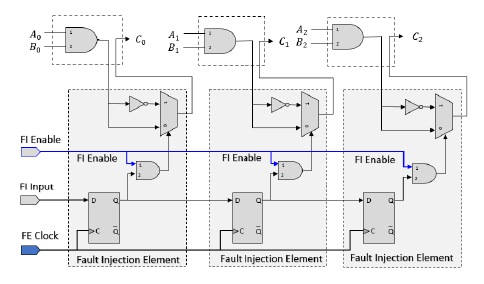
\includegraphics[width=0.9\linewidth]{assets/fish.png}
    \caption{Complete FISH Logic Circuit}
    \label{fig:complete_fish}
\end{figure}

The methodology proposed by Shandilya, Rahul and Sharma, R. demonstrates notably improved performance when compared to \textit{BUFIT} and \textit{SCFIT}, both of which are hardware-based fault injection techniques commonly used for reliability evaluation. \textit{BUFIT} primarily focuses on single-bit fault injection through direct modification of flip-flop states, offering simplicity, while lacking support for realistic multi-bit upset scenarios. On the other hand, \textit{SCFIT} introduces faults by targeting scan-chain elements, enabling structured fault insertion but at the cost of increased design intrusion and reduced flexibility. 


As illustrated in Figure \ref{fig:results_fish}, FISH achieves a significantly higher fault injection rate of \texttt{111.1 faults/s} compared to the rest of the injection methods tested.

\begin{figure}[htbp]
    \centering
    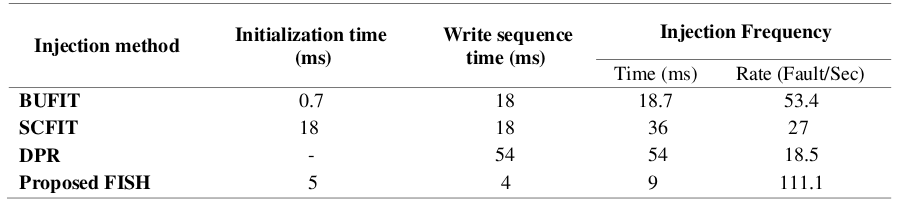
\includegraphics[width=0.9\linewidth]{assets/results_fish.png}
    \caption{Fault Injection Rate Comparison Between Techniques}
    \label{fig:results_fish}
\end{figure}

While the significantly higher injection rate of the proposed methodology plays an important factor in its usability, a more important role to consider is the hardware overhead needed for these implementations to function properly. As seen in Figure \ref{fig:fish_util}, which compares the utilization overhead of CLBs (Configurable Logic Blocks) and FFs (Flip Flops) of an FPGA programmed as an \textit{OR1200}, \textit{FISH} manages to stay relatively low in its usage requirements, comparing closely to the \textit{SCFIT} technique, which requires an extra 6\% of CLBs and 5.8\% of FFs to be added in addition to the FPGA target, while \textit{BUFIT}, shows a significantly less utilization overhead which is expected given its simplicity and lack of configurability. \\

\begin{figure}[htbp]
    \centering
    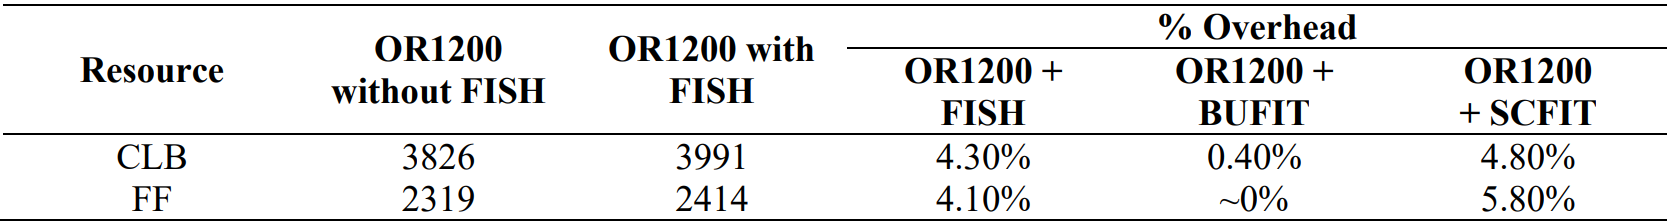
\includegraphics[width=0.9\linewidth]{assets/fish_util.png}
    \caption{Comparison of the Utilization of FI Techniques}
    \label{fig:fish_util}
\end{figure}

Overall, the experimental results indicate that FISH provides a more scalable and less intrusive solution for multi-bit fault injection, making it particularly suitable for reliability assessment of modern embedded and FPGA-based systems.